% Options for packages loaded elsewhere
\PassOptionsToPackage{unicode}{hyperref}
\PassOptionsToPackage{hyphens}{url}
\documentclass[
  10pt,
]{article}
\usepackage{xcolor}
\usepackage[margin=0.72in]{geometry}
\usepackage{amsmath,amssymb}
\setcounter{secnumdepth}{-\maxdimen} % remove section numbering
\usepackage{iftex}
\ifPDFTeX
  \usepackage[T1]{fontenc}
  \usepackage[utf8]{inputenc}
  \usepackage{textcomp} % provide euro and other symbols
\else % if luatex or xetex
  \usepackage{unicode-math} % this also loads fontspec
  \defaultfontfeatures{Scale=MatchLowercase}
  \defaultfontfeatures[\rmfamily]{Ligatures=TeX,Scale=1}
\fi
\usepackage{lmodern}
\ifPDFTeX\else
  % xetex/luatex font selection
  \setmainfont[]{Helvetica}
\fi
% Use upquote if available, for straight quotes in verbatim environments
\IfFileExists{upquote.sty}{\usepackage{upquote}}{}
\IfFileExists{microtype.sty}{% use microtype if available
  \usepackage[]{microtype}
  \UseMicrotypeSet[protrusion]{basicmath} % disable protrusion for tt fonts
}{}
\makeatletter
\@ifundefined{KOMAClassName}{% if non-KOMA class
  \IfFileExists{parskip.sty}{%
    \usepackage{parskip}
  }{% else
    \setlength{\parindent}{0pt}
    \setlength{\parskip}{6pt plus 2pt minus 1pt}}
}{% if KOMA class
  \KOMAoptions{parskip=half}}
\makeatother
\usepackage{longtable,booktabs,array}
\newcounter{none} % for unnumbered tables
\usepackage{calc} % for calculating minipage widths
% Correct order of tables after \paragraph or \subparagraph
\usepackage{etoolbox}
\makeatletter
\patchcmd\longtable{\par}{\if@noskipsec\mbox{}\fi\par}{}{}
\makeatother
% Allow footnotes in longtable head/foot
\IfFileExists{footnotehyper.sty}{\usepackage{footnotehyper}}{\usepackage{footnote}}
\makesavenoteenv{longtable}
\usepackage{graphicx}
\makeatletter
\newsavebox\pandoc@box
\newcommand*\pandocbounded[1]{% scales image to fit in text height/width
  \sbox\pandoc@box{#1}%
  \Gscale@div\@tempa{\textheight}{\dimexpr\ht\pandoc@box+\dp\pandoc@box\relax}%
  \Gscale@div\@tempb{\linewidth}{\wd\pandoc@box}%
  \ifdim\@tempb\p@<\@tempa\p@\let\@tempa\@tempb\fi% select the smaller of both
  \ifdim\@tempa\p@<\p@\scalebox{\@tempa}{\usebox\pandoc@box}%
  \else\usebox{\pandoc@box}%
  \fi%
}
% Set default figure placement to htbp
\def\fps@figure{htbp}
\makeatother
\setlength{\emergencystretch}{3em} % prevent overfull lines
\providecommand{\tightlist}{%
  \setlength{\itemsep}{0pt}\setlength{\parskip}{0pt}}
\usepackage{caption}
\captionsetup{font=small,skip=3pt}
\usepackage{titlesec}
\titlespacing*{\section}{0pt}{7pt}{3pt}
\titleformat*{\section}{\large\bfseries}
\setlength{\parskip}{3pt}
\setlength{\parindent}{0pt}
\renewcommand{\arraystretch}{1.05}
\usepackage{etoolbox}
\usepackage{needspace}
\AtBeginEnvironment{longtable}{\footnotesize}
\usepackage{bookmark}
\IfFileExists{xurl.sty}{\usepackage{xurl}}{} % add URL line breaks if available
\urlstyle{same}
% fallback for those not using the hyperref driver hyperxmp:
\makeatletter
\@ifundefined{xmpquote}{\newcommand{\xmpquote}[1]{#1}}{}
\makeatother
\hypersetup{
  pdftitle={When a Model Says ``the Words Mattered Most'': Testing Text--Audio Fusion Weights Against What Swapping an Input Does},
  pdfauthor={Team 47: T. Beede, A. Inamdar, J. Nagpal, A. Samandi, R. Sanchez, A. Kumar},
  hidelinks,
  pdfcreator={LaTeX via pandoc}}

\title{When a Model Says ``the Words Mattered Most'': Testing
Text--Audio Fusion Weights Against What Swapping an Input Does}
\author{Team 47: T. Beede, A. Inamdar, J. Nagpal, A. Samandi, R.
Sanchez, A. Kumar}
\date{CSCI 544 midterm report}

\begin{document}
\maketitle

\subsection{1. Why this matters, and what we
found}\label{why-this-matters-and-what-we-found}

A voice assistant reads ``Great, thanks.'' as joy. The developer opens
the debugging panel and sees \emph{text weight 0.9, audio weight 0.1},
and concludes that the tone of voice was ignored. Is that conclusion
safe? Many text+audio emotion models combine a text prediction and an
audio prediction with a learned weight, and papers read that weight as
how much each modality mattered. If the weight does not match what the
model actually does when an input changes, a developer will look in the
wrong place.

\textbf{Task.} Emotion recognition on MELD (Poria et al.~2019), dialogue
from the TV show \emph{Friends}: one utterance, its transcript and its
audio clip, goes in; one of seven emotions (anger, disgust, fear, joy,
neutral, sadness, surprise) comes out. We use the official split (9,989
/ 1,109 / 2,610 utterances) and report weighted and macro F1.
\textbf{The quantity under test} is a per-utterance weight \emph{w} in
(0, 1) that mixes the two predictions, p =
\emph{w}·p\textsubscript{text} + (1 − \emph{w})·p\textsubscript{audio}.
Reading it as ``\emph{w} above 0.5 means text mattered more'' is the
claim we check. ``Influence'' here means something measurable: how much
the model's output moves when that modality is replaced by another
utterance's.

\textbf{What we found.} In a balanced model, the weight's call agrees
with which modality's replacement moves the prediction more far beyond
the best trivial guess, \textbf{+20.8 points} over always answering
``text''. In a text-dominated model it adds nothing, \textbf{−0.9
points} (interval touching zero). Both models were built by us on MELD.
We explain why a weight can mislead (it ignores how unusual each
modality's prediction is) and show this follows exactly from the fusion
arithmetic. We do not attribute the contrast between the two models to
any single cause; that is the subject of the experiments planned in
Section 5.

\textbf{Research questions.} RQ1: how often does the weight's call match
the swap-test winner, compared with an always-text rule? RQ2: how does
this change as one modality dominates? RQ3 (from our proposal): does
agreement fall when text and audio express conflicting emotions? RQ1 and
RQ2 are answered preliminarily here; RQ3 is not yet tested.
\textbf{Hypotheses.} H1 (exploratory): the weight's gain over
always-text shrinks as one modality dominates. H2 (from the proposal,
prospective): agreement is lower on verified conflicting text--audio
pairs than on matched same-emotion controls.

\subsection{2. Related work: what is known, and what we
add}\label{related-work-what-is-known-and-what-we-add}

{\def\LTcaptype{none} % do not increment counter
\begin{longtable}[]{@{}
  >{\raggedright\arraybackslash}p{(\linewidth - 6\tabcolsep) * \real{0.1375}}
  >{\raggedright\arraybackslash}p{(\linewidth - 6\tabcolsep) * \real{0.3125}}
  >{\raggedright\arraybackslash}p{(\linewidth - 6\tabcolsep) * \real{0.1750}}
  >{\raggedright\arraybackslash}p{(\linewidth - 6\tabcolsep) * \real{0.3750}}@{}}
\toprule\noalign{}
\begin{minipage}[b]{\linewidth}\raggedright
Work
\end{minipage} & \begin{minipage}[b]{\linewidth}\raggedright
What is gated or intervened on
\end{minipage} & \begin{minipage}[b]{\linewidth}\raggedright
Gate weights checked against interventions?
\end{minipage} & \begin{minipage}[b]{\linewidth}\raggedright
How our audit differs
\end{minipage} \\
\midrule\noalign{}
\endhead
\bottomrule\noalign{}
\endlastfoot
Liu, Li, Meng 2020 & gates on feature vectors; claims ``interpretable
contribution weights'' (Sec. 3.6) & no & one scalar weight on class
probabilities, tested utterance by utterance \\
He, Xiao 2026 (LPGNet) & feature gates and softmax weights over
modalities; ``adaptively assigns importance to each modality'' & no
(whole-module ablation) & same \\
Hessel, Lee 2020 & EMAP: output averaged over other examples' values of
one input (image+text) & n/a: no gates; the intervention is the tool &
same averaging idea, read at one utterance's predicted class and
compared with the model's own weight \\
Jin et al.~2021 & per-instance modality saliency by masking, used to
weight distillation losses & n/a: masking saliency used for training; no
gate weights compared & real-utterance substitution; audits a weight
instead of training with scores \\
\end{longtable}
}

Gate values are already read as importance (Liu et al.; He and Xiao),
and substitution and masking are established tools (Hessel and Lee; Jin
et al.). We do not claim to have invented either. \textbf{Our
contribution is the audit that joins them:} for utterance-level
text+audio emotion models with a scalar late-fusion weight, we measure
how often the weight identifies the modality whose replacement matters
more, against a trivial constant rule, and we show when it stops adding
anything. To our knowledge, among the work we read, no paper tests a
fusion weight this way. Our gate is simpler than the published
feature-level gates, so our results do not transfer to them without
separate tests. Jain and Wallace (2019), Wiegreffe and Pinter (2019) and
Jacovi and Goldberg (2020) motivate the framing: define faithfulness
carefully, use trivial baselines, and make graded claims.

\subsection{3. Method in plain terms}\label{method-in-plain-terms}

\textbf{Models} (all built by us; pretrained encoders frozen, only small
linear heads and the gate trained). Each head outputs seven emotion
probabilities; the gate, a small network (one hidden layer of 128 units,
sigmoid output) reading a 384-d text embedding and the audio embedding,
outputs \emph{w}. Table 1 lists the three models. M3 is M5 without the
context stage; we introduce it because it has M5's encoders and strength
but judges each utterance alone, which the conflict experiment needs
(Section 5).

\begin{longtable}[]{@{}
  >{\raggedright\arraybackslash}p{(\linewidth - 10\tabcolsep) * \real{0.1546}}
  >{\raggedright\arraybackslash}p{(\linewidth - 10\tabcolsep) * \real{0.2165}}
  >{\raggedright\arraybackslash}p{(\linewidth - 10\tabcolsep) * \real{0.1753}}
  >{\raggedright\arraybackslash}p{(\linewidth - 10\tabcolsep) * \real{0.2577}}
  >{\raggedright\arraybackslash}p{(\linewidth - 10\tabcolsep) * \real{0.0515}}
  >{\raggedright\arraybackslash}p{(\linewidth - 10\tabcolsep) * \real{0.1443}}@{}}
\caption{Models. W-F1 and M-F1 are weighted and macro F1 (\%) of the
learned-gate model with the dev-fitted class-prior correction described
below. The published bcLSTM baseline is 59.25 weighted F1 and
DialogueRNN 60.25 (Poria et al.~2019); the comparison is descriptive,
not controlled, since our encoders are newer.}\tabularnewline
\toprule\noalign{}
\begin{minipage}[b]{\linewidth}\raggedright
Model
\end{minipage} & \begin{minipage}[b]{\linewidth}\raggedright
Text side
\end{minipage} & \begin{minipage}[b]{\linewidth}\raggedright
Audio side
\end{minipage} & \begin{minipage}[b]{\linewidth}\raggedright
Context
\end{minipage} & \begin{minipage}[b]{\linewidth}\raggedright
Gates
\end{minipage} & \begin{minipage}[b]{\linewidth}\raggedright
W-F1 / M-F1
\end{minipage} \\
\midrule\noalign{}
\endfirsthead
\toprule\noalign{}
\begin{minipage}[b]{\linewidth}\raggedright
Model
\end{minipage} & \begin{minipage}[b]{\linewidth}\raggedright
Text side
\end{minipage} & \begin{minipage}[b]{\linewidth}\raggedright
Audio side
\end{minipage} & \begin{minipage}[b]{\linewidth}\raggedright
Context
\end{minipage} & \begin{minipage}[b]{\linewidth}\raggedright
Gates
\end{minipage} & \begin{minipage}[b]{\linewidth}\raggedright
W-F1 / M-F1
\end{minipage} \\
\midrule\noalign{}
\endhead
\bottomrule\noalign{}
\endlastfoot
M1 balanced & MiniLM embedding, linear head & WavLM-large, all layers &
none & 10 & 58.8 / 41.1 \\
M3 strong, no context & RoBERTa-large, all layers & as M1 & none & 10 &
62.7 / 46.4 \\
M5 text-heavy & as M3 & as M3 & neighbouring utterances' first-stage
outputs (audio stage also uses following ones) & 3 & 63.6 / 46.5 \\
\end{longtable}

\textbf{Class-prior correction (plain English).} MELD is dominated by
neutral. Our heads are trained with class weights, which pushes
predictions toward rare emotions; the correction partly undoes that by
multiplying each emotion's fused probability by (its training
frequency)\textsuperscript{α} and renormalising, with α chosen on the
dev set (never on test; 0.25 for M1, 0.5 for M5). \emph{Illustrative
example (made-up numbers, three emotions instead of seven):} fused
probabilities neutral 0.38, joy 0.42, anger 0.20 and training
frequencies 0.50, 0.30, 0.20 (summing to one); with α = 0.25 the scores
are 0.320, 0.311, 0.134, which renormalise to neutral 0.418, joy 0.407,
anger 0.175, so the prediction moves from joy to neutral. All results
below that carry an F1 use this corrected rule.

\textbf{Swap test (plain English).} For one utterance we freeze the
emotion the model first predicted. To measure the text's influence, we
put in the text of another utterance, rerun the whole model (including
the gate), and record the probability of that same emotion. We do this
with every utterance in a pool of 8,004 training utterances (all of
them, no sampling; on average 8,003 valid text donors and 8,004 audio
donors per test utterance, excluding clips whose embedding is identical
to the explained utterance's), average the answers, and measure how far
the average sits from the original probability. Doing the same for audio
gives two numbers; the modality with the larger one ``mattered more''.
\emph{Illustrative example (made-up numbers):} the model says anger with
probability 0.68; averaging over text donors gives 0.64 (effect 0.04)
and over audio donors 0.50 (effect 0.18). Audio mattered more, even if
the weight said 0.8 for text, so the weight and the swap test disagree
on this utterance. \textbf{Agreement} is the share of test utterances
where the weight's call (text if \emph{w} \textgreater{} 0.5) equals the
swap winner. \textbf{Baseline:} always answering the modality that wins
most often, which here is ``text'' in every model (chosen on dev swaps,
so no test outcome selects it). \textbf{Gain} is agreement minus that
baseline. Intervals are 95\% from a bootstrap that resamples whole test
dialogues (1,000 draws).

\needspace{16\baselineskip}

\subsection{4. Results}\label{results}

\begin{longtable}[]{@{}
  >{\raggedright\arraybackslash}p{(\linewidth - 6\tabcolsep) * \real{0.4375}}
  >{\centering\arraybackslash}p{(\linewidth - 6\tabcolsep) * \real{0.0833}}
  >{\centering\arraybackslash}p{(\linewidth - 6\tabcolsep) * \real{0.0833}}
  >{\raggedright\arraybackslash}p{(\linewidth - 6\tabcolsep) * \real{0.3958}}@{}}
\caption{Swap-test results, primary rule (first two rows) and
sensitivity check. Intervals: dialogue-bootstrap.}\tabularnewline
\toprule\noalign{}
\begin{minipage}[b]{\linewidth}\raggedright
Model
\end{minipage} & \begin{minipage}[b]{\linewidth}\centering
Text swap larger
\end{minipage} & \begin{minipage}[b]{\linewidth}\centering
Weight agrees
\end{minipage} & \begin{minipage}[b]{\linewidth}\raggedright
Gain over always-text {[}95\% CI{]}
\end{minipage} \\
\midrule\noalign{}
\endfirsthead
\toprule\noalign{}
\begin{minipage}[b]{\linewidth}\raggedright
Model
\end{minipage} & \begin{minipage}[b]{\linewidth}\centering
Text swap larger
\end{minipage} & \begin{minipage}[b]{\linewidth}\centering
Weight agrees
\end{minipage} & \begin{minipage}[b]{\linewidth}\raggedright
Gain over always-text {[}95\% CI{]}
\end{minipage} \\
\midrule\noalign{}
\endhead
\bottomrule\noalign{}
\endlastfoot
M1 balanced & 52.8\% & 73.6\% & \textbf{+20.8} {[}18.5, 23.2{]} \\
M5 text-heavy & 92.9\% & 91.9\% & \textbf{−0.9} {[}−1.9, −0.0{]} \\
\emph{Sensitivity: swap on the uncorrected fused probability} & & & \\
M1 & 54.2\% & 75.4\% & +21.1 {[}18.8, 23.6{]} \\
M3 (strong, no context) & 92.8\% & 92.7\% & −0.1 {[}−0.6, +0.4{]} \\
M5 & 95.2\% & 93.6\% & −1.6 {[}−2.6, −0.6{]} \\
\end{longtable}

\begin{figure}
\centering
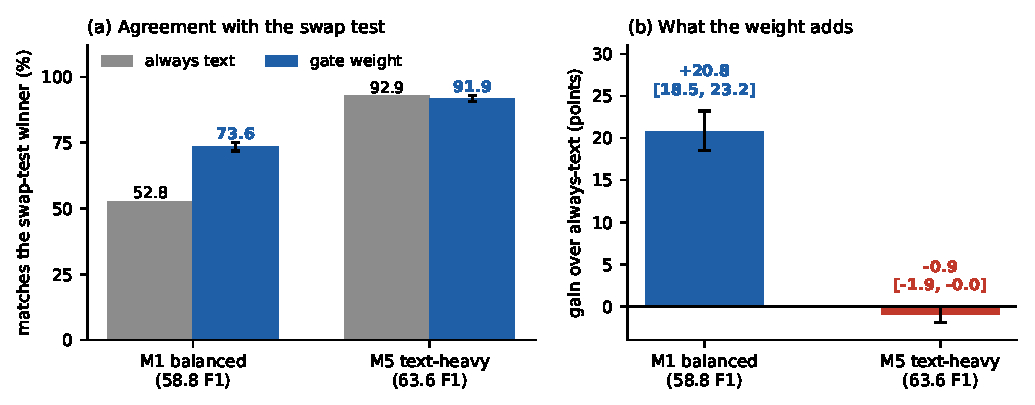
\includegraphics[width=1\linewidth,height=\textheight,keepaspectratio,alt={Corrected decision rule, primary measure. (a) How often a call matches the swap-test winner. (b) The weight's gain over always answering ``text'', with 95\% dialogue-bootstrap intervals.}]{../figures/fig7_gain_corrected_rule.pdf}
\caption{Corrected decision rule, primary measure. (a) How often a call
matches the swap-test winner. (b) The weight's gain over always
answering ``text'', with 95\% dialogue-bootstrap intervals.}
\end{figure}

\textbf{Finding 1: the weight is informative in the balanced model.} It
matches the swap winner in 73.6\% of utterances, against 52.8\% for
always-text, and its ranking of how much more text than audio mattered
correlates at 0.70 with the measured gap (Spearman, 95\% interval 0.68
to 0.72). \textbf{Finding 2: it adds nothing in the text-heavy model.}
Text wins about 93\% of the time and the weight does no better than
always answering text (−0.9 points, interval touching zero: no evidence
of an advantage, and at most a small disadvantage). When audio did win
(4.8\% of utterances, uncorrected probability), the weight said so in
53.9\% of those cases, and was right in 38.3\% of the audio calls it
made. M2, a strong-text model without context, shows the same pattern
(text wins 97.1\%; −0.4 {[}−0.7, −0.1{]}, uncorrected probability).

\textbf{Why a weight can mislead.} Replacing a modality with an average
replacement changes the output by roughly \emph{weight × how different
its prediction is from the average replacement's prediction}. A high
weight therefore means little if the modality's prediction already looks
like a typical replacement. With the gate held fixed this identity is
exact (it matches the swap winner in 100\% of utterances), and the
weight times this ``distinctiveness'' has rank correlation 0.97 with the
measured gap, against 0.72 for the weight alone (M1, uncorrected
probability). \textbf{Because it is the swap's own arithmetic, this
explains the gap; it is not independent evidence of importance.} Letting
the gate re-weight per replacement changes the winner for 4 to 8\% of
utterances and lowers the gain by 2 to 4 points relative to a frozen
gate, but even with the gate frozen M5's gain is only +1.0 to +1.3, so
we do not call re-weighting the cause of the text-heavy result.

\textbf{Robustness.} Dropping the 42 test utterances with shared audio
changes no gain by more than 0.2 points. Averaging absolute
per-replacement changes instead gives the same signs for M1, M2, M3 and
M5. The two models differ in encoders, strength, context and the number
of trained gates (10 for M1 and M3, 3 for M5), so the contrast between
them is a finding to explain, not an established cause.

\subsection{5. Status against the proposal, and what we test
next}\label{status-against-the-proposal-and-what-we-test-next}

\textbf{Conflict experiment (RQ3).} The proposal's hypothesis, that
agreement falls when text and audio express different emotions, is
untested. We have written and frozen the protocol before running any
model on a constructed pair, and prepared a 100-pair package that three
reviewers will annotate blind to the dataset labels (differing MELD
labels do not guarantee that the emotions sound or read as conflicting).
We will compare, per text, a verified conflicting pairing with a matched
same-emotion control, with weight-versus-swap agreement as the outcome
and Holm correction over two models. With about 100 verified items only
large effects (roughly 10 to 20 points) are detectable, so a null result
will be reported as inconclusive. \textbf{M3 replaces M5} here because a
constructed pair has no coherent neighbouring utterances for M5's
context stage; M3 has the same encoders and a similar text dominance
(text wins 92.8\%, uncorrected probability), so M1 (balanced) and M3
(strong text) are run under one identical procedure.

\begin{longtable}[]{@{}
  >{\raggedright\arraybackslash}p{(\linewidth - 2\tabcolsep) * \real{0.4267}}
  >{\raggedright\arraybackslash}p{(\linewidth - 2\tabcolsep) * \real{0.5733}}@{}}
\caption{Proposal milestones and their status.}\tabularnewline
\toprule\noalign{}
\begin{minipage}[b]{\linewidth}\raggedright
Proposal commitment
\end{minipage} & \begin{minipage}[b]{\linewidth}\raggedright
Status
\end{minipage} \\
\midrule\noalign{}
\endfirsthead
\toprule\noalign{}
\begin{minipage}[b]{\linewidth}\raggedright
Proposal commitment
\end{minipage} & \begin{minipage}[b]{\linewidth}\raggedright
Status
\end{minipage} \\
\midrule\noalign{}
\endhead
\bottomrule\noalign{}
\endlastfoot
Baselines on official splits, weighted and macro F1 & done (Table 1) \\
Effects of removing or changing a modality & done, extended: swap test;
silence and mean replacement run on an earlier model only \\
Gate weight versus confidence-based signal & partly: confidence rule
analysed, its agreement is partly structural \\
Spearman and ranking agreement & done \\
Gradient / SHAP signals (optional) & not started \\
Conflict test & protocol frozen, annotation pending, no results \\
\end{longtable}

\textbf{Next.} Oct 28 to Nov 2: annotation and adjudication of the pilot
package (proceed only if reviewer agreement is acceptable). Nov 3 to 17:
build, verify and run the test-split conflict study on M1 and M3; ablate
what the gate sees (it reads MiniLM text embeddings even where the text
head reads RoBERTa). Nov 18 to 24: a controlled series that degrades one
modality in a single architecture with several trained heads, and
robustness to matched replacements. Dec: final report.

\textbf{Limitations.} Two model families we built on one dataset; heads
are shared across gates, so intervals reflect test-set sampling, not
head-training variance; random replacements create unnatural pairs
(Hessel and Lee note the same for EMAP); the gate's design differs from
published feature-level gates. Code, protocols and result tables are in
the project repository (corrected-rule protocol committed as 4f4c662
before its run; conflict protocol frozen in 5f878c7 and amended before
annotation in ff55b48).

\subsection{References}\label{references}

\footnotesize

Poria et al.~(2019). MELD: A multimodal multi-party dataset for emotion
recognition in conversations. \emph{ACL}.

Liu, P., Li, K., Meng, H. (2020). Group gated fusion on attention-based
bidirectional alignment for multimodal emotion recognition.
\emph{Interspeech 2020} (arXiv:2201.06309).

He, Z., Xiao, Y. (2026). LPGNet: A lightweight network with parallel
attention and gated fusion for multimodal emotion recognition.
\emph{Circuits, Systems, and Signal Processing} 45(9):7634--7652.
doi:10.1007/s00034-026-03547-w (arXiv:2508.08925; quotations here are
from the arXiv v1 text).

Hessel, J., Lee, L. (2020). Does my multimodal model learn cross-modal
interactions? It's harder to tell than you might think! \emph{EMNLP}
(arXiv:2010.06572).

Jin, W., Sanjabi, M., Nie, S., Tan, L., Ren, X., Firooz, H. (2021). MSD:
Saliency-aware knowledge distillation for multimodal understanding.
\emph{Findings of EMNLP 2021} (arXiv:2101.01881).

Jain, S., Wallace, B. C. (2019). Attention is not explanation.
\emph{NAACL}. Wiegreffe, S., Pinter, Y. (2019). Attention is not not
explanation. \emph{EMNLP-IJCNLP}. Jacovi, A., Goldberg, Y. (2020).
Towards faithfully interpretable NLP systems: How should we define and
evaluate faithfulness? \emph{ACL}.

\end{document}
